\documentclass[titlepage]{article}

\usepackage{
    geometry,
    multicol,
    pdfpages
}

\geometry{
    letterpaper,
    margin=1in
}

\setlength{\columnsep}{0.25in}

\title{
    \textbf{
        CSCE 221 --- 200 \\
        Programming Assignment 4 \\
        Final Report
    }
}

\author{
    James Corder Guy \\
    Nathan Powell
}

\date{
    \today
}

\begin{document}
    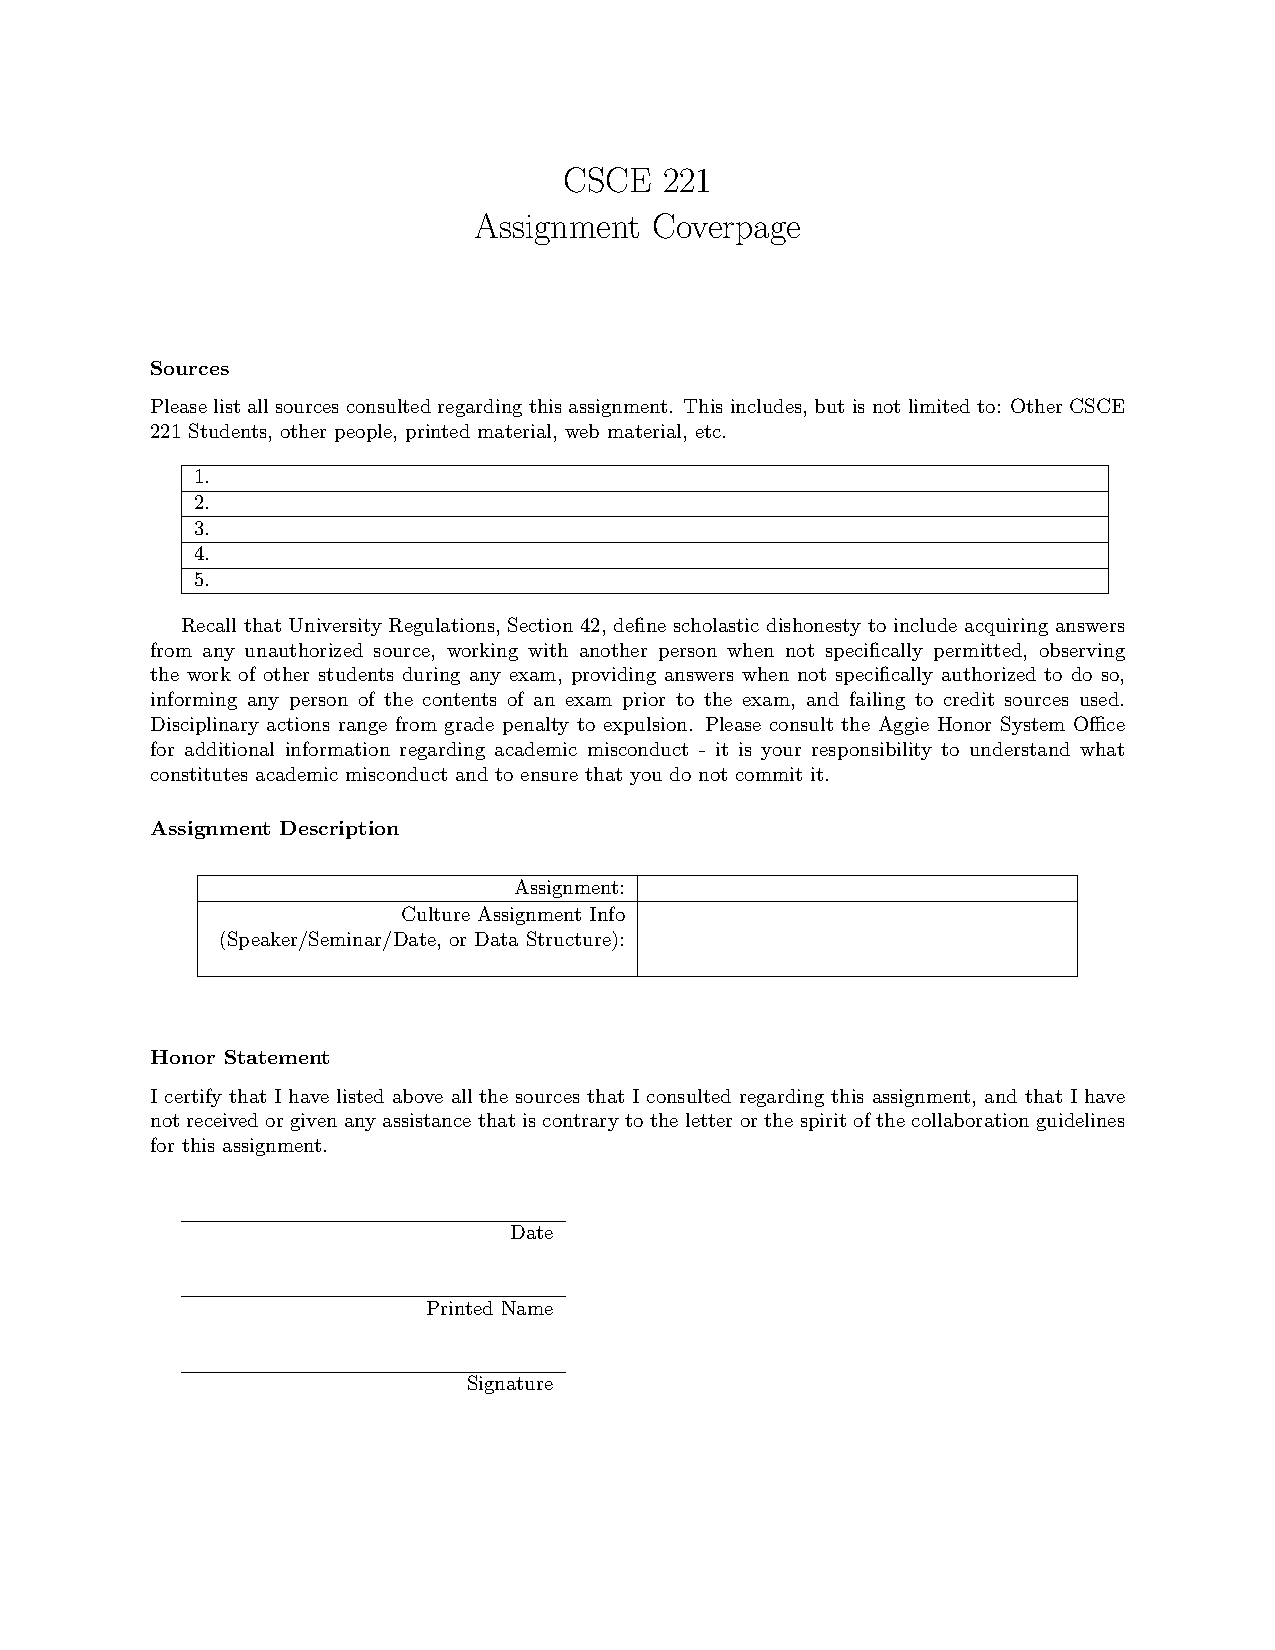
\includepdf[pages={-}]{./coverpage.pdf}
    \maketitle
    \begin{multicols*}{2}
        \section{Introduction}
            For this project, we implemented a fully-functional graph data structure, along with breadth-first search and Kruskal's minimum spanning tree algrorithms.
        \section{Implementation Details}
            \subsection{Graph}
                The graph was implemented using a map of vertices, a master map of edges, and an adjacency edge map for each vertex. The vertex map keys the vertices by their identifiers, and each element contains a pointer to its corresponding vertex. Each vertex is assigned a unique identifier number corresponding to the number at which it was inputted, and also a list of edges that connect to it. Both the master and the adjacency edge maps key the edges by the vertex identifier pairs that they connect, and each element contains a pointer to its corresponding edge. Each edge contains the descriptors of the two verticies it connects, and its weight. All edges are directed; in order to insert an undirected edge, two edges going in opposite directions between the same two vertices are inserted.
            \subsection{Input/Output}
                The graph pulls its initial vertices and edges from a file, reading in first the number of vertices, then the number of edges. It then reads in the next $n$ lines, where $n$ is the number of vertices, and initializes them as vertices in the vertex container. The graph then reads in the remaining lines as edges, with each line having three values, in the order of source vertex, destination vertex, and weight.
            \subsection{Breadth-First Search}

            \subsection{Kruskal's Algorithm}
                Kruskal's Algorithm was used to find the minimum spanning tree of the input graph. The edges in the minimum spanning tree were copied into a parent map. To start, the algorithm read all the edges in the graph into a multimap, keying the edges by weight. Next, the first and last keys in the multimap are checked; if they are the same, then every edge in the map must have the same weight; therefore, every spanning tree is a minimum spanning tree. If not, the algorithm continues and sets up containers known as clusters; these represent the vertices linked together by Krusr ekal's algorithm that will form the minimum spanning tree. Another container that holds pointers to each cluster is initialized for constant access to each cluster. Every vertex is then inserted into its own cluster, and the algorithm begins to iterate through every edge in the multimap, comparing the vertices it connects; if they are not in the same cluster, that edge is added to the parent map, and the smaller cluster is merged into the larger cluster, though the now empty smaller cluster is not deleted; doing so would reindex the remaining clusters, invalidating all of the pointers to the clusters. This process repeats until there are n-1 edges in the parent map, with n being the number of vertices in the graph.
        \section{Theoretical Analysis}
            \subsection{Graph}
            \subsection{Input/Output}
            \subsection{Breadth-First Search}
            \subsection{Minimum Spanning Tree}
            \subsection{Kruskal's Algorithm}
                Kruskal's Algorithm should run in O((n+m)logn) time, because each vertex will be merged at most log(n) times, resulting in O(nlogn) time, because smaller clusters are always merged into larger clusters, and there will be at most m removals from the edge multimap (because there are m edges in total), resulting in O(mlogn) time, because each union operation on the edge's vertices takes O(logn) time. Therefore, the total running time of Kruskao's Algorithm is O((n+m)logn) time.
        \section{Experimental Analysis}
            \subsection{Testing Hardware}
                Specifications of Nathan's system, used for testing Kruskal's Algorithm: \\ \\
                \begin{tabular}{r l}
                CPU:    & Intel i5-2430M @ 2.40GHz \\
                RAM:    & 8GB \\
                OS:     & Linux Mint 17.3 Cinnamon \\
                Kernel: & 3.19.0-32 \\
                \end{tabular} \\ \\
                \noindent
                Specifications of Corder's system, used for testing BFS: \\ \\
                \begin{tabular}{r l}
                CPU:    & Intel i5-4210U @ 2.7GHz \\
                RAM:    & 8GB \\
                OS:     & Arch Linux \\
                Kernel: & 4.5.1-1 \\
                \end{tabular} \\ \\

            \subsection{Testing Procedure}
                Input Size: \\ \\
                \begin{tabular}{r l}
                Complete:   & $2^{11}$ \\
                Mesh:       & $2^{15}$ \\
                Random:     & $2^{14}$ \\
                \end{tabular}

            \subsection{Results}
            \subsection{Big-O Constants}
        \section{Results and Discussion}
        \section{Team Contributions}
            \subsection{Graph}
                \begin{tabular}{l l}
                    Nathan: & iterators, containers, inserters, erasers \\
                    Corder: & accessors, mutators
                \end{tabular}
            \subsubsection{Vertex}
                \begin{tabular}{l l}
                    Nathan: & adjacency list \\
                    Corder: & iterators, accessors, data members
                \end{tabular}
            \subsubsection{Edge}
                \begin{tabular}{l l}
                Corder: & iterators, accessors, data members
                \end{tabular}
            \subsubsection{I/O}
                \begin{tabular}{l l}
                   Nathan: & input \\
                   Corder: & output
                \end{tabular}
            \subsection{Algorithms}
                \begin{tabular}{l l}
                    Nathan: & Kruskal's \\
                    Corder: & BFS
                \end{tabular}
        \section{Conclusion}
    \end{multicols*}
\end{document}
